\documentclass[tikz,border=10pt]{standalone}
\usepackage[T1]{fontenc}
\usepackage{lmodern}
\usepackage[table]{xcolor}
\usepackage{tikz}
\usetikzlibrary{arrows.meta,positioning}

\definecolor{umlheader}{RGB}{220, 235, 252}
\renewcommand{\arraystretch}{1.35}

\tikzset{
  umlclass/.style={
    draw=none,
    align=left,
    inner sep=0pt,
    outer sep=0pt,
    font=\sffamily\small
  },
  inherit/.style={
    -{Triangle[open,length=3.40mm,width=2.80mm]},
    line width=0.5pt,
    shorten <=-0.4pt,
    shorten >=-0.4pt
  }
}

\begin{document}
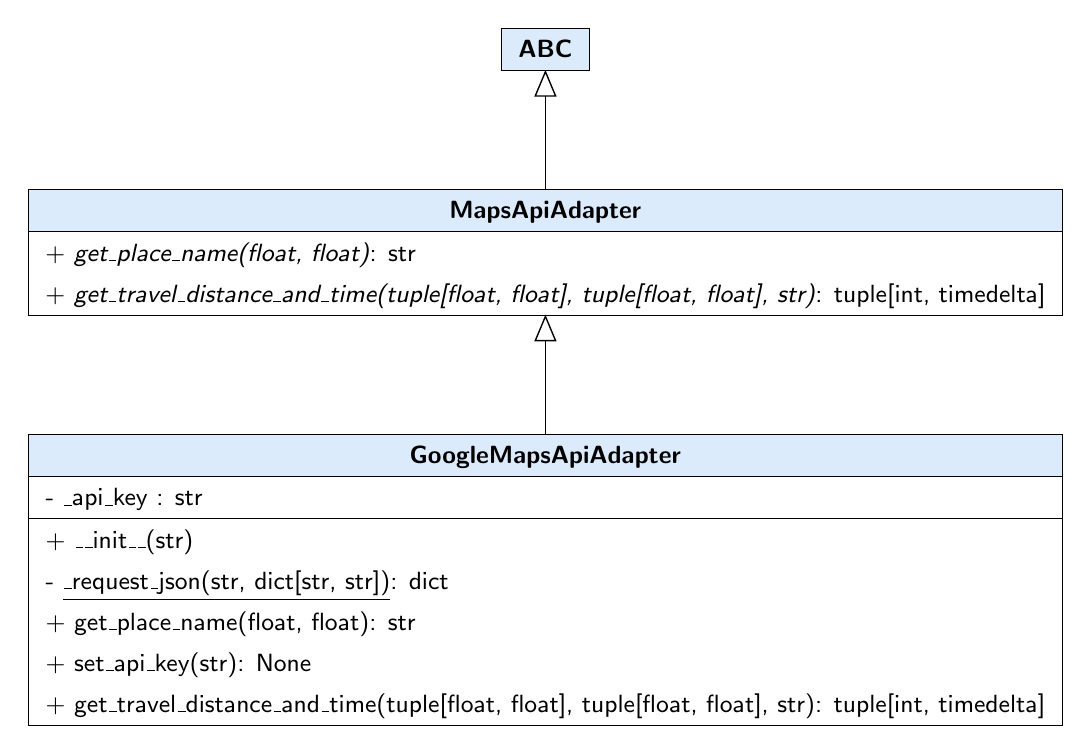
\begin{tikzpicture}
\node[umlclass] (c0) at (0.00,0) {\begin{tabular}{|l|}
\hline
\rowcolor{umlheader}\multicolumn{1}{|c|}{\textbf{ABC}} \\
\hline
\end{tabular}};
\node[umlclass,below=1.50cm of c0.south,xshift=+0.00cm] (c2) {\begin{tabular}{|l|}
\hline
\rowcolor{umlheader}\multicolumn{1}{|c|}{\textbf{MapsApiAdapter}} \\
\hline
+ \textit{get\_place\_name(float, float)}: str \\
+ \textit{get\_travel\_distance\_and\_time(tuple[float, float], tuple[float, float], str)}: tuple[int, timedelta] \\
\hline
\end{tabular}};
\node[umlclass,below=1.50cm of c2.south,xshift=+0.00cm] (c1) {\begin{tabular}{|l|}
\hline
\rowcolor{umlheader}\multicolumn{1}{|c|}{\textbf{GoogleMapsApiAdapter}} \\
\hline
- \_api\_key : str \\
\hline
+ \_\_init\_\_(str) \\
- \underline{\_request\_json(str, dict[str, str])}: dict \\
+ get\_place\_name(float, float): str \\
+ set\_api\_key(str): None \\
+ get\_travel\_distance\_and\_time(tuple[float, float], tuple[float, float], str): tuple[int, timedelta] \\
\hline
\end{tabular}};

\draw[inherit] (c1.north) -- (c2.south);
\draw[inherit] (c2.north) -- (c0.south);
\end{tikzpicture}
\end{document}
